\section{Phân tích thiết kế hệ thống}

\subsection{Bài toán nghiệp vụ}

Hệ thống hỗ trợ người dùng
hỏi đáp pháp luật Việt Nam,
phân tích tài liệu
và đàm thoại trực tiếp thời gian thực
với trợ lý ảo pháp lý.
Dựa trên thiết kế hướng miền (DDD),
bài toán lớn được chia làm
các miền phụ (Subdomain)
với các chức năng như sau:

\begin{figure}[H]
\centering
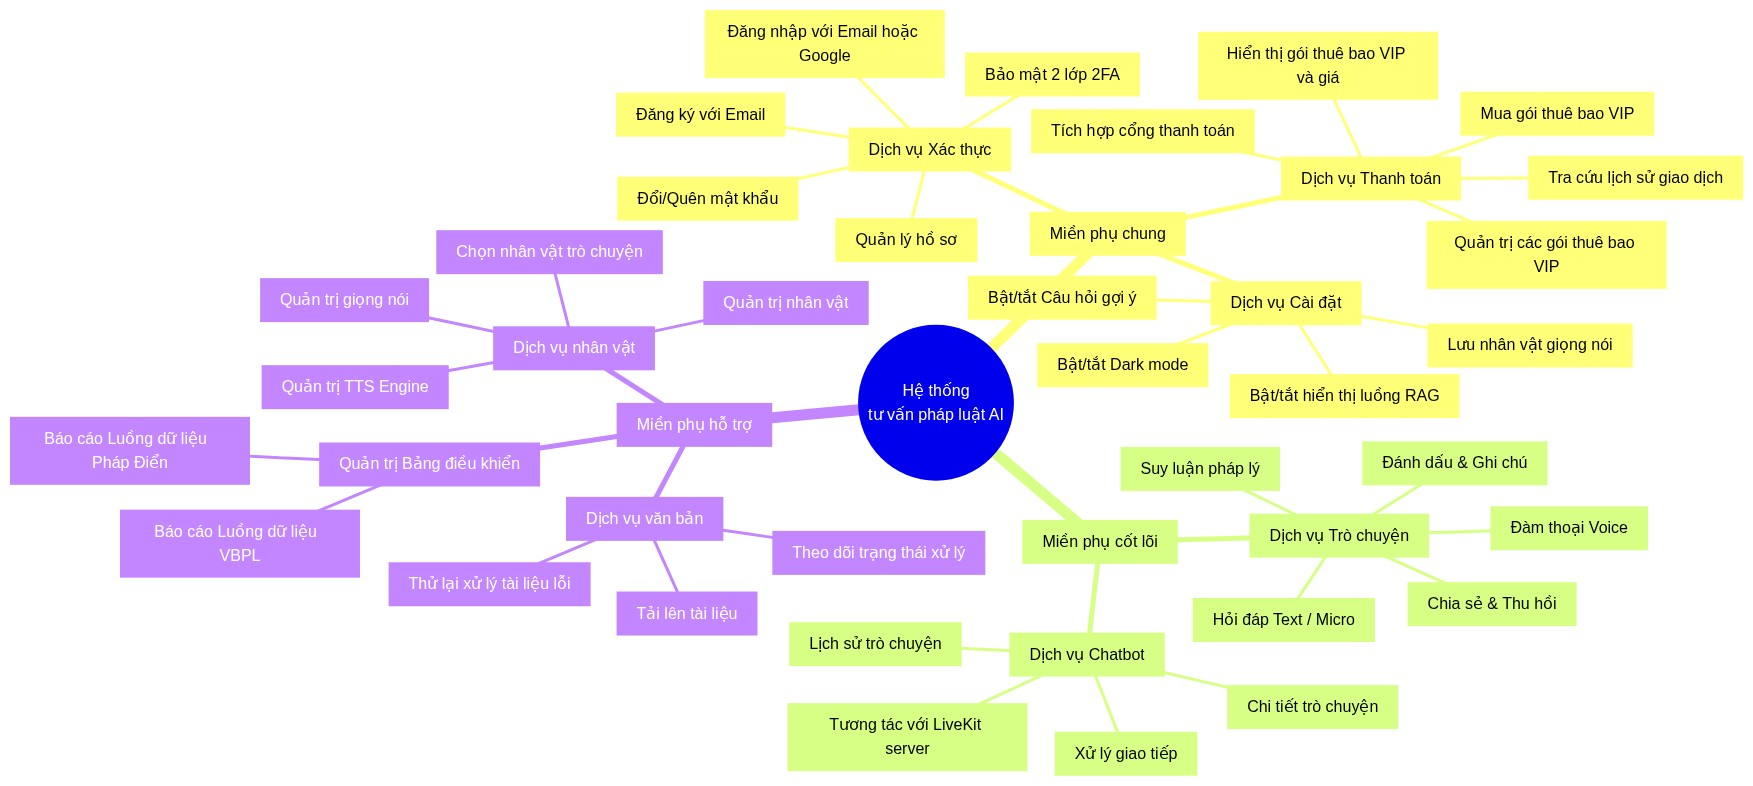
\includegraphics[scale = 0.25]{pictures/SubDomainMindMap.png}
\caption{Sơ đồ tổng quan SubDomain}
\end{figure}

\subsubsection{Miền phụ cốt lõi (Core Subdomain)}

Miền phụ cốt lõi
là phần quan trọng
và có giá trị nhất của hệ thống.
Miền phụ cốt lõi
giúp phân biệt các doanh nghiệp
và làm cho các doanh nghiệp có giá trị.
Miền phụ cốt lõi
tập trung vào mục tiêu
và yêu cầu của khách hàng với doanh nghiệp,
từ đó quyết định sự thành công của doanh nghiệp.
Vì vậy, mỗi doanh nghiệp
luôn tìm cách thực hiện những điều khác biệt
trong các miền phụ cốt lõi này để đạt được lợi thế so với đối thủ cạnh tranh.

% TODO: Subdomain-Core.tex
% TODO: Subdomain-Core.tex
% TODO: Subdomain-Core.tex

\input{contents/SubDomain-Core.tex} % \paragraph{Đặc điểm người dùng hệ thống}

Miền phụ cốt lõi
là nơi diễn ra các luồng xử lý phức tạp
và quyết định đến mức độ hài lòng của người dùng.

\subsubsection{Miền phụ hỗ trợ (Supporting Subdomain)}

Các miền phụ cốt lõi phụ thuộc
vào các miền phụ hỗ trợ.
Miền phụ hỗ trợ cung cấp các dịch vụ
để miền phụ cốt lõi hoạt động hiệu quả.
Tuy nhiên, miền phụ hỗ trợ không đòi hỏi mức độ phức tạp cao về logic nghiệp vụ.

% TODO: SubDomain-Supporting.tex
% TODO: SubDomain-Supporting.tex
% TODO: SubDomain-Supporting.tex

\input{contents/SubDomain-Supporting.tex} % \paragraph{Đặc điểm người dùng hệ thống}

Miền phụ hỗ trợ giúp miền phụ cốt lõi không bị phình to.
Tách nhỏ việc quản lý nhân vật, giọng nói
và quá trình xử lý tài liệu tiêu tốn nhiều tài nguyên hệ thống.

\subsubsection{Miền phụ chung (Generic Subdomain)}

Miền phụ chung
cung cấp các giải pháp có sẵn
mà doanh nghiệp có thể mua, thuê.
Miền phụ chung
có thể được tìm thấy trên nhiều ngành.
Doanh nghiệp không thể đạt được bất kỳ lợi thế cạnh tranh so
với đối thủ bằng cách thực hiện những điều khác biệt trong miền phụ chung.

% TODO: SubDomain-Generic.tex
% TODO: SubDomain-Generic.tex
% TODO: SubDomain-Generic.tex

\input{contents/SubDomain-Generic.tex} % \paragraph{Đặc điểm người dùng hệ thống}

Việc áp dụng các giải pháp có sẵn
như Supabase (Auth) hay Neon API (Settings)
là một chiến lược thông minh
để rút ngắn thời gian phát triển.
Đặc biệt là việc tích hợp 2FA,
điều kiện tiên quyết
cho các hệ thống xử lý hợp đồng
và dữ liệu pháp luật mang tính nhạy cảm.

Sơ đồ phân rã chức năng

\begin{figure}[H]
\centering
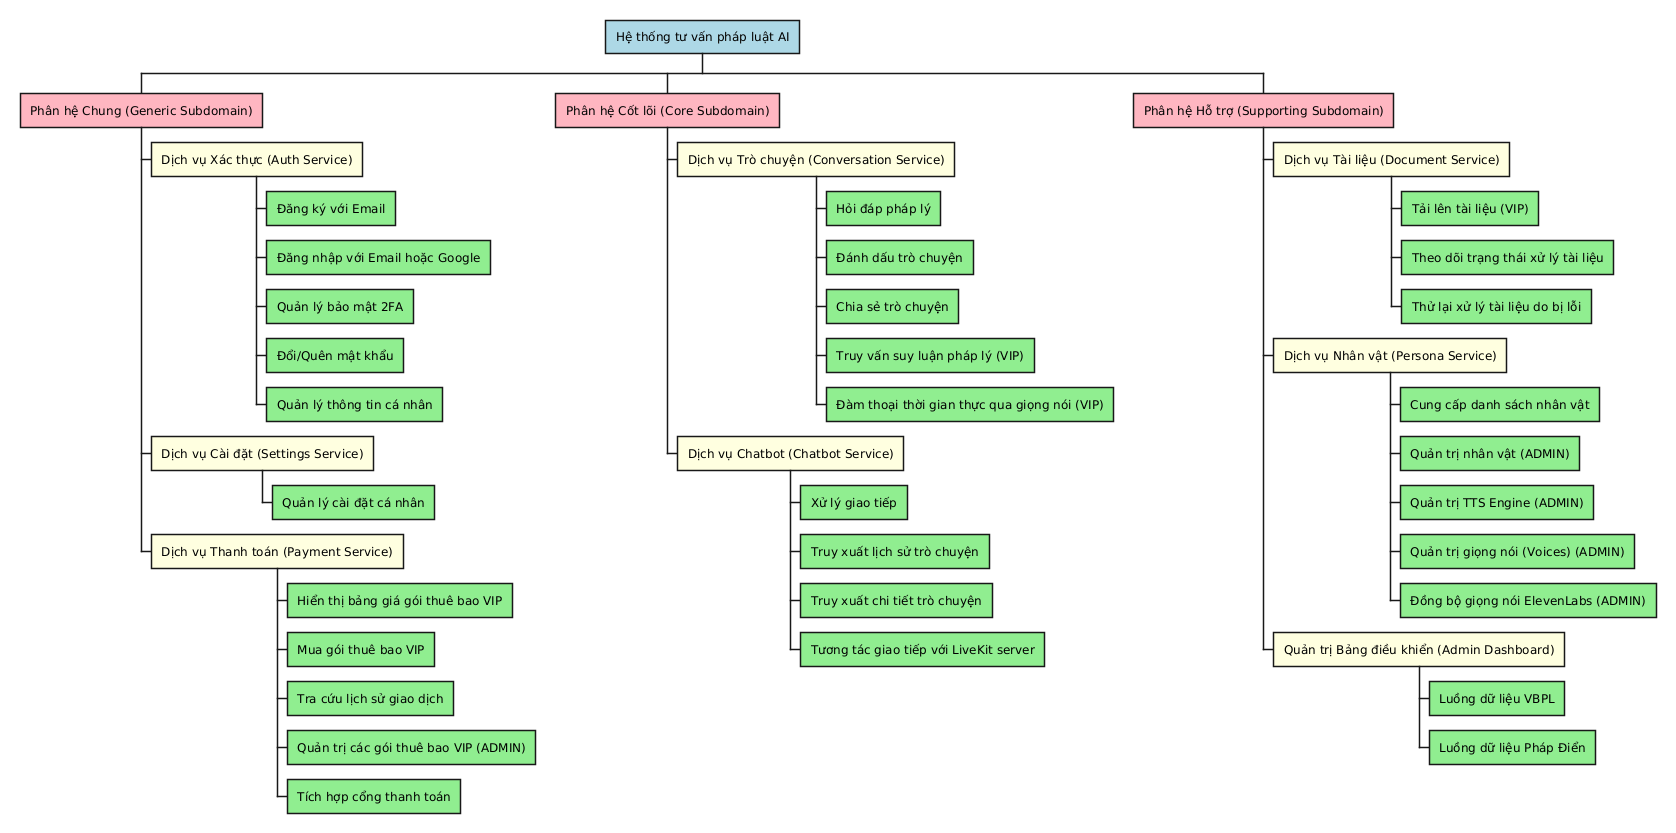
\includegraphics[scale = 0.18]{pictures/BFD.png}
\caption{Sơ đồ phân rã chức năng}
\end{figure}
